\documentclass[12pt,a4paper]{article}

% ==================== PACKAGES ====================
\usepackage[utf8]{inputenc}
\usepackage[T1]{fontenc}
\usepackage{mathptmx} % Times New Roman font matching Word template
\usepackage[margin=2.54cm, bottom=2.8cm]{geometry}
\usepackage{array}
\usepackage{tabularx}
\usepackage{multirow}
\usepackage{longtable}
\usepackage{xcolor}
\usepackage{listings}
\usepackage{fancyhdr}
\usepackage{lastpage}
\usepackage{enumitem}
\usepackage{tikz}
\usetikzlibrary{shapes.multipart, arrows.meta, positioning, calc}
\usepackage{hyperref}

% ==================== COLORS & STYLES ====================
\definecolor{wordblue}{HTML}{4F81BD}
\definecolor{codebg}{HTML}{F8F9FA}
\definecolor{codeframe}{HTML}{D1D5DB}
\definecolor{javakeyword}{HTML}{0033B3}
\definecolor{javastring}{HTML}{067D17}
\definecolor{javacomment}{HTML}{8C8C8C}

\lstdefinestyle{javastyle}{
    language=Java,
    basicstyle=\ttfamily\small,
    keywordstyle=\color{javakeyword}\bfseries,
    stringstyle=\color{javastring},
    commentstyle=\color{javacomment}\itshape,
    backgroundcolor=\color{codebg},
    frame=single,
    rulecolor=\color{codeframe},
    breaklines=true,
    tabsize=4,
    showstringspaces=false,
    aboveskip=8pt,
    belowskip=8pt
}

% ==================== FOOTER: "Page X of Y" ====================
\pagestyle{fancy}
\fancyhf{}
\renewcommand{\headrulewidth}{0pt}
\fancyfoot[C]{\textcolor{wordblue}{\fontfamily{phv}\selectfont\small Page \textbf{\thepage} of \textbf{\pageref*{LastPage}}}}

\setlength{\parindent}{0pt}
\setlength{\parskip}{6pt}

\begin{document}

% ==================== DOCUMENT TITLE ====================
\begin{center}
    {\fontsize{24}{28}\selectfont\bfseries LIBRARY MANAGEMENT SYSTEM\par}
\end{center}
\vspace{0.3cm}

% ==================== GROUP INFO TABLE ====================
\renewcommand{\arraystretch}{1.6}
\begin{tabular}{|>{\raggedleft\arraybackslash\bfseries}p{4.2cm}|>{\bfseries}p{10.8cm}|}
    \hline
    \multicolumn{2}{|c|}{\rule{0pt}{0.7cm}\fontsize{15}{18}\selectfont\bfseries Group: Group 01} \\[0.2cm]
    \hline
    Group Members &
    $<$Member 1 Name$>$ - $<$SE20xxx1$>$ \newline
    $<$Member 2 Name$>$ - $<$SE20xxx2$>$ \newline
    $<$Member 3 Name$>$ - $<$SE20xxx3$>$ \newline
    $<$Member 4 Name$>$ - $<$SE20xxx4$>$ \\
    \hline
    Lecturer & $<$Lecturer Name$>$ \\
    \hline
    Class & $<$SE20xx$>$ \\
    \hline
\end{tabular}

\vspace{0.6cm}

% ==================== TASK ASSIGNMENT TABLE ====================
\renewcommand{\arraystretch}{1.5}
\begin{tabular}{|p{0.6cm}|p{2.3cm}|p{3.2cm}|p{2.3cm}|p{5.6cm}|}
    \hline
    \textbf{\#} &
    \textcolor{wordblue}{\textbf{Student ID}} &
    \textcolor{wordblue}{\textbf{Full Name}} &
    \textcolor{wordblue}{\textbf{Completion}} &
    \textcolor{wordblue}{\textbf{Tasks Performed}} \\
    \hline
    \textbf{\textit{1}} &
    \textbf{\textit{SE20xxx1}} &
    \textbf{\textit{Member 1 (Leader)}} &
    \textbf{\textit{100\%}} &
    \textbf{\textit{User, Member, IMemberDAO, MemberDAO, MemberManagement, addMember, updateMember, deleteMember, filterByTier, Members.txt}} \\
    \hline
    \textbf{\textit{2}} &
    \textbf{\textit{SE20xxx2}} &
    \textbf{\textit{Member 2}} &
    \textbf{\textit{100\%}} &
    \textbf{\textit{Book, TextBook, ReferenceBook, IBookDAO, BookDAO, BookManagement, calculatePrice, rateBook, recommendSimilarBooks, reserveBook, Books.txt}} \\
    \hline
    \textbf{\textit{3}} &
    \textbf{\textit{SE20xxx3}} &
    \textbf{\textit{Member 3}} &
    \textbf{\textit{100\%}} &
    \textbf{\textit{BorrowRecord, IBorrowDAO, BorrowDAO, BorrowManagement, borrowBooks, returnBooks, extendLoan, reportLostOrDamaged, exportReceiptToFile}} \\
    \hline
    \textbf{\textit{4}} &
    \textbf{\textit{SE20xxx4}} &
    \textbf{\textit{Member 4}} &
    \textbf{\textit{100\%}} &
    \textbf{\textit{DataInput, DataValidation, Menu, printAsciiBarChart, FileManager, Program, displaySystemDashboard, exportSystemSummaryReport}} \\
    \hline
\end{tabular}

\vspace{0.6cm}

% ====================================================================
% MILESTONE 1 (Lab01 - Week 3)
% ====================================================================
{\fontsize{16}{20}\selectfont\bfseries Milestone 1(Lab01 - Week 3) Template --- Requirements \& Initial Class Diagram\par}

\hspace{0.8cm}{\itshape\bfseries Document Title: Milestone 1 -- Requirements Analysis, Decomposition \& Abstraction\par}

\textbf{1. Project Title}

\textit{Library Management System}

\textbf{2. Problem Description (5--7 sentences)}

``In this project, I aim to design a system that manages multi-category books, library members, and borrowing/returning transactions in a university library. The main users will be librarians and library administrators who oversee daily catalog updates, reader registration, and book circulation. The system will help solve the problem of manual record-keeping errors, difficulty in tracking overdue loans, inaccurate book stock counts, and lack of member credit evaluation. The key functions include book inventory management (\texttt{TextBook} and \texttt{ReferenceBook}), member management with automated membership tiers (\texttt{SILVER}, \texttt{GOLD}, \texttt{VIP}) and reputation points, loan processing with due-date extension and lost/damaged book compensation, star ratings with smart book recommendations, FIFO reservation queues, and console ASCII bar charts. This project will apply OOP and Computational Thinking to decompose the problem and build an efficient solution.''

\textbf{3. Functional Requirements}

\begin{itemize}[leftmargin=1.2cm]
    \item \textbf{Book Management:} Add new books (\texttt{TextBook}, \texttt{ReferenceBook}), delete books, edit book information, search books (by ID, keyword, price range, or category), sort books (by calculated price ascending or publish year descending), rate books ($1\text{--}5\star$), recommend top 3 similar books, and reserve out-of-stock books via a FIFO waiting queue.
    \item \textbf{Member Management:} Add, edit, delete, search, and sort library members; automatically classify membership tiers (\texttt{VIP} $\ge 150$ pts, \texttt{GOLD} $100\text{--}149$ pts, \texttt{SILVER} $< 100$ pts) to apply borrowing limits ($10 / 7 / 5$ books) and fee discounts ($25\% / 10\% / 0\%$), and auto-lock cards when reputation drops below $0$.
    \item \textbf{Borrow \& Return Management:} Create borrow tickets with stock deduction, process book returns with stock restoration and overdue fine calculation ($5,000\text{ VND/day/book}$), extend active loans ($+7\text{ days}$, max $1$ time), penalize lost/damaged books ($150\%$ of polymorphic book price), notify the first reserved member upon book return, and export transaction receipts (\texttt{Receipt\_<ID>.txt}).
    \item \textbf{System Dashboard, Visual Analytics \& File I/O:} Display console ASCII bar charts (Inventory, Member Tiers, Top Borrowed Books), synchronize UTF-8 text files (\texttt{Books.txt}, \texttt{Members.txt}, \texttt{BorrowRecords.txt}), and export \texttt{Library\_Summary\_Report.txt}.
\end{itemize}

\textbf{4. System Decomposition (CT: Decomposition)}

``The system can be divided into the following modules:
\begin{enumerate}[leftmargin=1.5cm]
    \item \textbf{Core.Entities Module:} Represents domain entities (\texttt{User}, \texttt{Member}, \texttt{Book}, \texttt{TextBook}, \texttt{ReferenceBook}, \texttt{BorrowRecord}) with encapsulated states and polymorphic behaviors.
    \item \textbf{DataObjects.DAO Module:} Manages object collections (\texttt{ArrayList}) and UTF-8 file persistence through standardized interfaces (\texttt{IBookDAO}, \texttt{IMemberDAO}, \texttt{IBorrowDAO}, \texttt{BookDAO}, \texttt{MemberDAO}, \texttt{BorrowDAO}, \texttt{FileManager}).
    \item \textbf{BusinessObject.UI Module:} Handles interactive console menus and tabular displays (\texttt{Program}, \texttt{BookManagement}, \texttt{MemberManagement}, \texttt{BorrowManagement}).
    \item \textbf{Utilities Module:} Provides reusable input handling, regex validation, and ASCII bar chart rendering (\texttt{DataInput}, \texttt{DataValidation}, \texttt{Menu}).
\end{enumerate}
Each module has a clear responsibility in the system.''

\textbf{5. Identified Classes (CT: Abstraction)}

\renewcommand{\arraystretch}{1.4}
\begin{longtable}{p{3.0cm} p{5.5cm} p{6.2cm}}
    \textbf{\fontfamily{phv}\selectfont\small Class Name} &
    \textbf{\fontfamily{phv}\selectfont\small Attributes} &
    \textbf{\fontfamily{phv}\selectfont\small Methods} \\
    \hline
    \texttt{User} \newline \textit{(abstract)} &
    \texttt{\# id: String} \newline
    \texttt{\# name: String} \newline
    \texttt{\# phone: String} \newline
    \texttt{\# email: String} &
    \texttt{+ getId() / setId(String)} \newline
    \texttt{+ getName() / setName(String)} \newline
    \texttt{+ getPhone() / setPhone(String)} \newline
    \texttt{+ getEmail() / setEmail(String)} \newline
    \texttt{+ displayInfo(): void (abstract)} \\
    \hline
    \texttt{Member} &
    \texttt{- membershipDate: String} \newline
    \texttt{- status: String} \newline
    \texttt{- reputationPoints: int} &
    \texttt{+ getMembershipTier(): String} \newline
    \texttt{+ getTierDiscountRate(): double} \newline
    \texttt{+ getMaxBorrowLimit(): int} \newline
    \texttt{+ adjustReputationPoints(int): void} \newline
    \texttt{+ displayInfo(): void} \newline
    \texttt{+ toFileString(): String} \\
    \hline
    \texttt{Book} \newline \textit{(abstract)} &
    \texttt{\# bookId, title, author, publisher: String} \newline
    \texttt{\# publishYear, quantity, ratingCount: int} \newline
    \texttt{\# basePrice, ratingSum: double} \newline
    \texttt{\# reservationQueue: List<String>} &
    \texttt{+ calculatePrice(): double (abstract)} \newline
    \texttt{+ displayInfo(): void (abstract)} \newline
    \texttt{+ toFileString(): String (abstract)} \newline
    \texttt{+ addRating(int): void} \newline
    \texttt{+ getAverageRating(): double} \newline
    \texttt{+ addReservation(String): boolean} \newline
    \texttt{+ popNextReservation(): String} \\
    \hline
    \texttt{TextBook} &
    \texttt{- status: String ("New"/"Old")} \newline
    \texttt{- subject: String} &
    \texttt{+ calculatePrice(): double} \newline
    \texttt{+ displayInfo(): void} \newline
    \texttt{+ toFileString(): String} \\
    \hline
    \texttt{ReferenceBook} &
    \texttt{- tax: double} \newline
    \texttt{- field: String} &
    \texttt{+ calculatePrice(): double} \newline
    \texttt{+ displayInfo(): void} \newline
    \texttt{+ toFileString(): String} \\
    \hline
    \texttt{BorrowRecord} &
    \texttt{- recordId: String} \newline
    \texttt{- member: Member} \newline
    \texttt{- borrowedBooks: List<Book>} \newline
    \texttt{- borrowDate, dueDate, returnDate: LocalDate} \newline
    \texttt{- status: String} \newline
    \texttt{- extensionCount: int} \newline
    \texttt{- compensationFee: double} &
    \texttt{+ calculateFine(): double} \newline
    \texttt{+ calculateTotalBorrowFee(): double} \newline
    \texttt{+ calculateDefaultCompensationFee(): double} \newline
    \texttt{+ extendDueDate(int): boolean} \newline
    \texttt{+ isOverdue(): boolean} \newline
    \texttt{+ displayInfo(): void} \newline
    \texttt{+ toFileString(): String} \\
    \hline
\end{longtable}

\textbf{6. Relationships between real-world objects}

\begin{center}
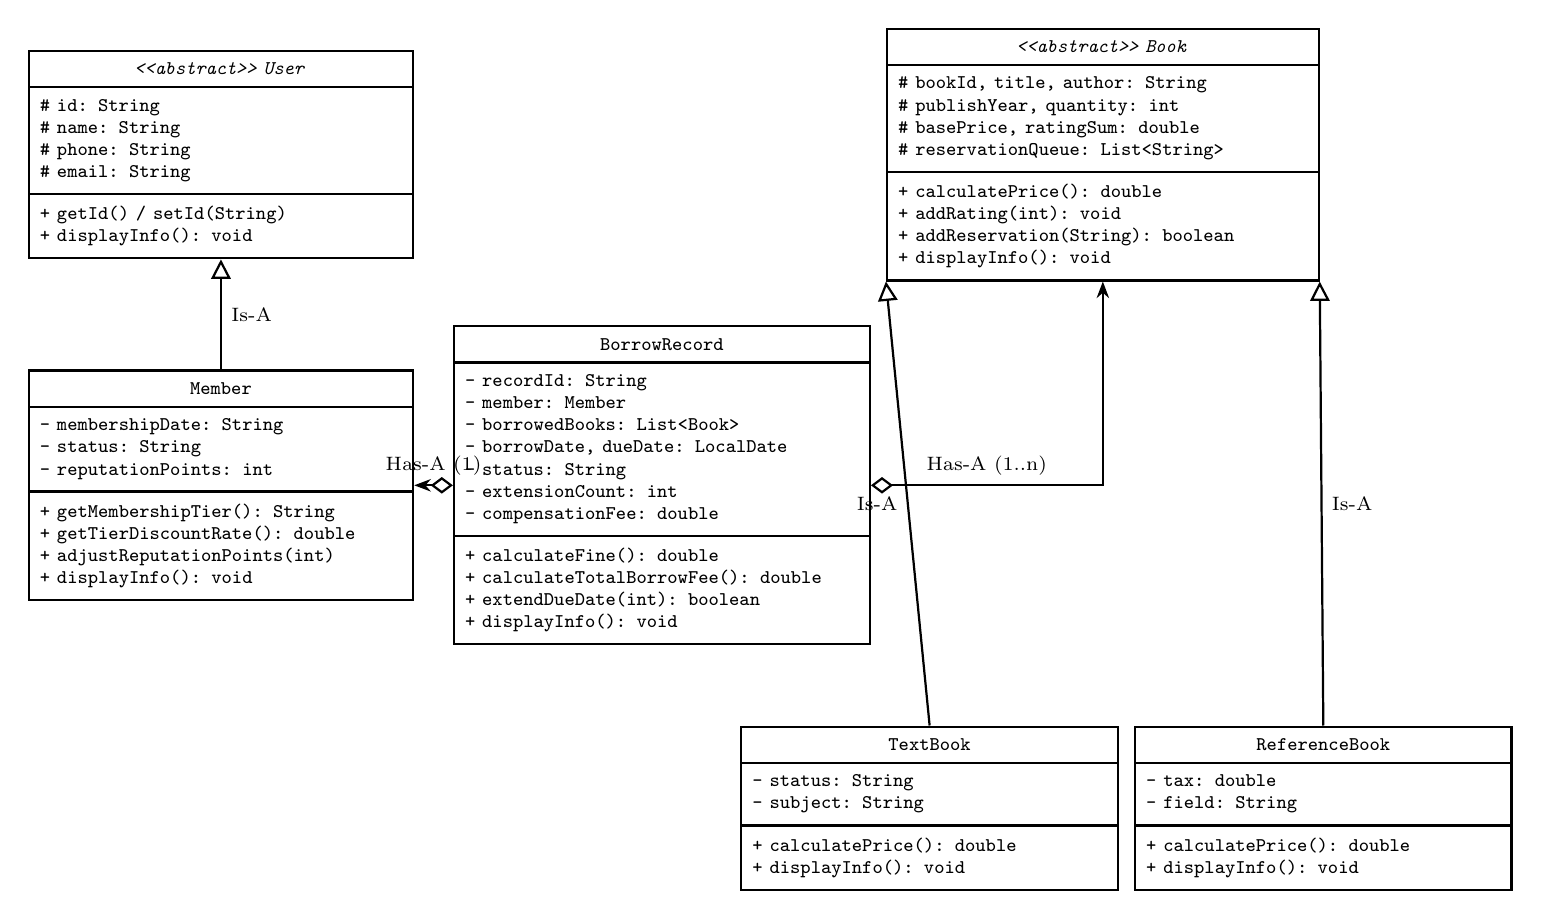
\begin{tikzpicture}[
    classbox/.style={
        rectangle split, rectangle split parts=3,
        draw=black, thick, fill=white,
        font=\ttfamily\scriptsize, align=left,
        text width=4.6cm, inner sep=4pt
    },
    inherit/.style={-{Triangle[open, length=7pt, width=7pt]}, thick},
    aggreg/.style={{Diamond[open, length=8pt, width=6pt]}-{Stealth[length=6pt]}, thick}
]
    \node[classbox] (user) at (0, 0) {
        \centerline{\textbf{\textit{<<abstract>> User}}}
        \nodepart{second}
        \# id: String\\
        \# name: String\\
        \# phone: String\\
        \# email: String
        \nodepart{third}
        + getId() / setId(String)\\
        + displayInfo(): void
    };

    \node[classbox] (member) at (0, -4.2) {
        \centerline{\textbf{Member}}
        \nodepart{second}
        - membershipDate: String\\
        - status: String\\
        - reputationPoints: int
        \nodepart{third}
        + getMembershipTier(): String\\
        + getTierDiscountRate(): double\\
        + adjustReputationPoints(int)\\
        + displayInfo(): void
    };

    \node[classbox, text width=5.0cm] (borrow) at (5.6, -4.2) {
        \centerline{\textbf{BorrowRecord}}
        \nodepart{second}
        - recordId: String\\
        - member: Member\\
        - borrowedBooks: List<Book>\\
        - borrowDate, dueDate: LocalDate\\
        - status: String\\
        - extensionCount: int\\
        - compensationFee: double
        \nodepart{third}
        + calculateFine(): double\\
        + calculateTotalBorrowFee(): double\\
        + extendDueDate(int): boolean\\
        + displayInfo(): void
    };

    \node[classbox, text width=5.2cm] (book) at (11.2, 0) {
        \centerline{\textbf{\textit{<<abstract>> Book}}}
        \nodepart{second}
        \# bookId, title, author: String\\
        \# publishYear, quantity: int\\
        \# basePrice, ratingSum: double\\
        \# reservationQueue: List<String>
        \nodepart{third}
        + calculatePrice(): double\\
        + addRating(int): void\\
        + addReservation(String): boolean\\
        + displayInfo(): void
    };

    \node[classbox, text width=4.5cm] (textbook) at (9.0, -8.3) {
        \centerline{\textbf{TextBook}}
        \nodepart{second}
        - status: String\\
        - subject: String
        \nodepart{third}
        + calculatePrice(): double\\
        + displayInfo(): void
    };

    \node[classbox, text width=4.5cm] (refbook) at (14.0, -8.3) {
        \centerline{\textbf{ReferenceBook}}
        \nodepart{second}
        - tax: double\\
        - field: String
        \nodepart{third}
        + calculatePrice(): double\\
        + displayInfo(): void
    };

    \draw[inherit] (member.north) -- (user.south) node[midway, right, font=\scriptsize\rmfamily] {Is-A};
    \draw[inherit] (textbook.north) -- (book.south west) node[midway, left, font=\scriptsize\rmfamily] {Is-A};
    \draw[inherit] (refbook.north) -- (book.south east) node[midway, right, font=\scriptsize\rmfamily] {Is-A};
    \draw[aggreg] (borrow.west) -- (member.east) node[midway, above, font=\scriptsize\rmfamily] {Has-A (1)};
    \draw[aggreg] (borrow.east) -| (book.south) node[pos=0.25, above, font=\scriptsize\rmfamily] {Has-A (1..n)};
\end{tikzpicture}
\end{center}

\textbf{7. Encapsulation Evidence (Code Snippets)}

\begin{lstlisting}[style=javastyle]
public class Member extends User {
    // 1. Private attributes (Data Hiding)
    private String membershipDate;
    private String status;           // "Active" or "Inactive"
    private int reputationPoints;    // Default: 100 points (GOLD tier)

    // 2. Constructor chaining with superclass User
    public Member(String id, String name, String phone, String email,
                  String membershipDate, String status, int reputationPoints) {
        super(id, name, phone, email);
        this.membershipDate = membershipDate;
        this.status = status;
        this.reputationPoints = reputationPoints;
    }

    // 3. Getters & Setters with encapsulated business rules
    public int getReputationPoints() { return reputationPoints; }
    public void setReputationPoints(int reputationPoints) {
        this.reputationPoints = reputationPoints;
    }
    public void adjustReputationPoints(int delta) {
        this.reputationPoints += delta;
        if (this.reputationPoints < 0) {
            this.status = "Inactive"; // Auto-lock card if reputation < 0
        }
    }
}
\end{lstlisting}

\textbf{8. Reflection (4--6 sentences)}

``In this milestone, I learned that decomposition helps me break down complex tasks into manageable parts such as separating domain entities, data access objects, user interfaces, and validation utilities. I also practiced abstraction by identifying the essential classes needed in the system (\texttt{User}, \texttt{Member}, \texttt{Book}, \texttt{TextBook}, \texttt{ReferenceBook}, and \texttt{BorrowRecord}) while omitting unnecessary physical details. Describing the \texttt{Is-A} inheritance relationships and \texttt{Has-A} aggregation links between \texttt{BorrowRecord}, \texttt{Member}, and \texttt{Book} clarified how real-world library transactions work. This analysis will guide the next milestone where I implement encapsulation and \texttt{ArrayList} collection managers.''

\vspace{0.5cm}

% ====================================================================
% MILESTONE 2 (Lab 02 - Week 5)
% ====================================================================
{\fontsize{16}{20}\selectfont\bfseries Milestone 2(Lab 02 - Week 5) Template --- Encapsulation \& Basic Oparators\par}

{\itshape\bfseries Document Title: Milestone 2 -- Pattern Recognition\par}

\textbf{1. Summary of Progress (3--5 sentences)}

\textit{``In this milestone, most objects require Create, Read (display information), Update, and Delete (CRUD) operations and search information. As a result, the project uses \texttt{ArrayList<Book>}, \texttt{ArrayList<Member>}, and \texttt{ArrayList<BorrowRecord>} inside DAO classes to manage collections of objects dynamically. Furthermore, input validation and exception handling were implemented in \texttt{DataInput} and \texttt{DataValidation} to ensure that all objects remain valid throughout their lifecycle.''}

\textbf{2. Implemented management Classes Overview}

\hspace{0.5cm}\textbf{\textit{Name class:}} \textit{BookDAO (implements IBookDAO)}

\hspace{0.5cm}\textbf{\textit{Description:}} \textit{The BookDAO class is implemented in the project to manage the collection of books (\texttt{List<Book>}) in the library. This class provides basic operations such as adding new books, updating book information, deleting books, searching for books by ID/keyword/price range/type, sorting, rating stars, recommending similar books, and managing the FIFO reservation queue.}

\hspace{0.5cm}\textbf{\textit{Basic operator specifications:}}

\hspace{0.5cm}\textbf{\textit{Add a new book (addBook):}}
\begin{quote}
\textbf{\textit{Begin}}\\
\hspace*{0.5cm}\textit{Step 1: The user selects the book category (1 = TextBook, 2 = ReferenceBook) and inputs book information such as: bookId, title, author, publisher, publishYear, basePrice, quantity, and subclass attributes.}\\
\hspace*{0.5cm}\textit{Step 2: Validate inputted data using \texttt{DataValidation.isValidBookId(id)} (\texttt{\^{}B\textbackslash d\{3,\}\$}), check \texttt{findById(id) == null} to prevent duplicate IDs, and verify positive numeric ranges.}\\
\hspace*{0.5cm}\textit{Step 3: Instantiate \texttt{new TextBook(...)} or \texttt{new ReferenceBook(...)}, add the object to \texttt{bookList}, and invoke \texttt{saveToFile()} to persist into \texttt{Books.txt}.}\\
\textbf{\textit{End}}
\end{quote}

\hspace{0.5cm}\textbf{\textit{Name class:}} \textit{MemberDAO (implements IMemberDAO)}

\hspace{0.5cm}\textbf{\textit{Description:}} \textit{The MemberDAO class manages \texttt{List<Member> memberList}. It provides operations to register new members, update member status/reputation, delete members, search by ID or name, sort by name or reputation points, and filter by membership tier (\texttt{VIP}, \texttt{GOLD}, \texttt{SILVER}).}

\hspace{0.5cm}\textbf{\textit{Name class:}} \textit{BorrowDAO (implements IBorrowDAO)}

\hspace{0.5cm}\textbf{\textit{Description:}} \textit{The BorrowDAO class manages \texttt{List<BorrowRecord> recordList}. It handles borrowing books, returning books, extending due dates ($+7$ days), reporting lost/damaged books ($150\%$ compensation), and exporting receipts.}

\hspace{0.5cm}\textbf{\textit{Borrow books operation (borrowBooks):}}
\begin{quote}
\textbf{\textit{Begin}}\\
\hspace*{0.5cm}\textit{Step 1: Input \texttt{recordId} (\texttt{BRxxx}), \texttt{memberId} (\texttt{Mxxx}), list of \texttt{bookIds}, and \texttt{borrowDays}.}\\
\hspace*{0.5cm}\textit{Step 2: Validate that the member exists, has \texttt{"Active"} status, and does not exceed their tier borrow limit (\texttt{VIP: 10}, \texttt{GOLD: 7}, \texttt{SILVER: 5}).}\\
\hspace*{0.5cm}\textit{Step 3: Verify that every selected book exists and has \texttt{quantity > 0} (if \texttt{quantity == 0}, offer to join the FIFO \texttt{reservationQueue}).}\\
\hspace*{0.5cm}\textit{Step 4: Deduct book stock by 1 (\texttt{b.setQuantity(b.getQuantity() - 1)}), create \texttt{BorrowRecord}, apply tier discount, and save \texttt{BorrowRecords.txt} and \texttt{Books.txt}.}\\
\textbf{\textit{End}}
\end{quote}

\textbf{3. Encapsulation Evidence (Code Snippets)}

\begin{lstlisting}[style=javastyle]
public class BookDAO implements IBookDAO {
    // Encapsulated private collection of books
    private List<Book> bookList;
    private final String FILE_NAME = "Books.txt";

    @Override
    public boolean addBook(Book book) {
        if (book == null || findById(book.getBookId()) != null) {
            return false; // Prevent null or duplicate Book ID
        }
        bookList.add(book);
        saveToFile();
        return true;
    }

    @Override
    public Book findById(String bookId) {
        for (int i = 0; i < bookList.size(); i++) {
            Book b = bookList.get(i);
            if (b.getBookId().equalsIgnoreCase(bookId.trim())) {
                return b;
            }
        }
        return null;
    }
}
\end{lstlisting}

\textbf{4. Explanation of Abstraction / Pattern Recognition}

``I noticed that several classes share common method patterns such as \texttt{add()}, \texttt{update()}, \texttt{delete()}, \texttt{findById()}, \texttt{getAll()}, \texttt{loadFromFile()}, and \texttt{saveToFile()}. Based on these patterns, I designed standardized DAO interfaces (\texttt{IBookDAO}, \texttt{IMemberDAO}, and \texttt{IBorrowDAO}) and a shared \texttt{FileManager} class so that all managers follow the exact same structure. This helped improve the clarity, consistency, and reusability of the code across all four team members.''

\textbf{5. Challenges and Solutions}

``One challenge I faced was handling invalid user input on the console (such as entering letters instead of numbers for book price or publish year) and preventing invalid negative quantities inside entity objects. I solved it by encapsulating all \texttt{Scanner} reads inside \texttt{Utilities.DataInput} with \texttt{try-catch} validation loops and adding guard conditions inside entity setters (\texttt{setBasePrice}, \texttt{setQuantity}). This helped me better understand encapsulation and defensive programming.''

\textbf{6. Reflection (4--6 sentences)}

``In Milestone 2, implementing encapsulation and pattern recognition taught me how to protect internal \texttt{ArrayList} data structures from unauthorized external modification. By exposing only well-defined CRUD and search methods through DAO interfaces, we ensured that business rules such as unique IDs and non-negative stock quantities are never bypassed. Writing step-by-step pseudocode before coding complex workflows like book borrowing and smart recommendations also helped our group avoid logical bugs. Finally, recognizing recurring CRUD patterns allowed all four members to build consistent management classes.''

\vspace{0.5cm}

% ====================================================================
% MILESTONE 3 (Lab03 - Week 7)
% ====================================================================
{\fontsize{16}{20}\selectfont\bfseries Milestone 3 (Lab03 - Week 7) Template --- Inheritance \& Polymorphism\par}

\hspace{1.2cm}{\itshape\bfseries Document Title: Milestone 3 - Hierarchy \& Polymorphism,\par}
\hspace{4.8cm}{\itshape\bfseries - Generalization (Advanced Abstraction)\par}

\textbf{1. Summary of New Additions}

``In this milestone, I created a class hierarchy using inheritance (\texttt{User} $\rightarrow$ \texttt{Member} and \texttt{Book} $\rightarrow$ \texttt{TextBook}, \texttt{ReferenceBook}) and implemented polymorphism by overriding abstract methods (\texttt{calculatePrice()}, \texttt{displayInfo()}, and \texttt{toFileString()}). This helps the system handle different types of objects using a common interface.''

\textbf{2. Class Hierarchy Design (CT: Generalization)}

``The parent class is \textbf{\texttt{Book}} (abstract superclass for publications) and \textbf{\texttt{User}} (abstract superclass for people).\\
The child classes are \textbf{\texttt{TextBook}} and \textbf{\texttt{ReferenceBook}} (inheriting from \texttt{Book}), and \textbf{\texttt{Member}} (inheriting from \texttt{User}).\\
The shared attributes include \textbf{\texttt{bookId, title, author, publisher, publishYear, basePrice, quantity, ratingSum, ratingCount, reservationQueue}} in \texttt{Book}, and \textbf{\texttt{id, name, phone, email}} in \texttt{User}.\\
Each subclass adds unique behaviors such as \textbf{\texttt{TextBook}} calculating price based on condition (\texttt{New} = $100\%$, \texttt{Old} = $50\%$ of \texttt{basePrice}), \textbf{\texttt{ReferenceBook}} calculating price with import tax and a $15,000\text{ VND}$ hardcover fee (\texttt{basePrice + basePrice * tax + 15000}), and \textbf{\texttt{Member}} computing dynamic tiers (\texttt{VIP}/\texttt{GOLD}/\texttt{SILVER}) and fee discounts from \texttt{reputationPoints}.''

\textbf{3. UML Hierarchy Diagram}

\begin{center}
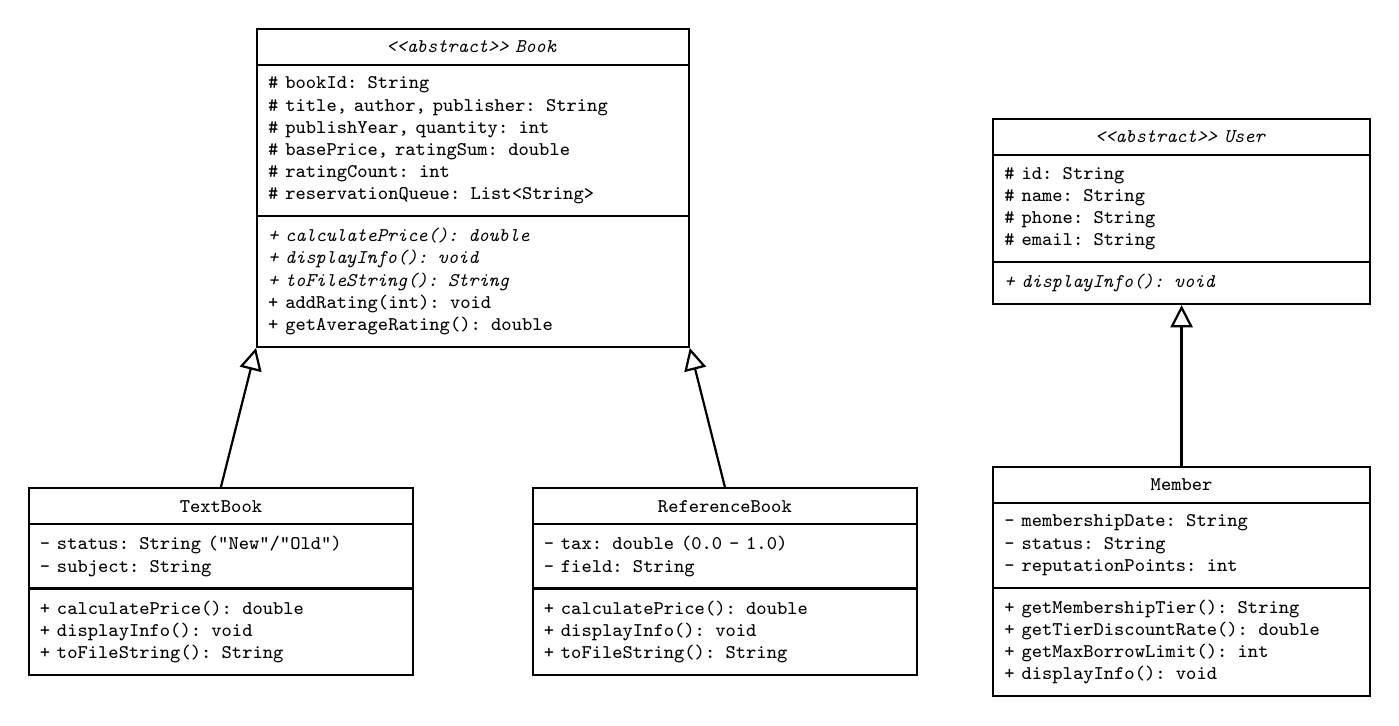
\begin{tikzpicture}[
    classbox/.style={
        rectangle split, rectangle split parts=3,
        draw=black, thick, fill=white,
        font=\ttfamily\scriptsize, align=left,
        text width=5.2cm, inner sep=4pt
    },
    inherit/.style={-{Triangle[open, length=8pt, width=8pt]}, thick}
]
    \node[classbox] (book) at (0, 0) {
        \centerline{\textbf{\textit{<<abstract>> Book}}}
        \nodepart{second}
        \# bookId: String\\
        \# title, author, publisher: String\\
        \# publishYear, quantity: int\\
        \# basePrice, ratingSum: double\\
        \# ratingCount: int\\
        \# reservationQueue: List<String>
        \nodepart{third}
        \textit{+ calculatePrice(): double}\\
        \textit{+ displayInfo(): void}\\
        \textit{+ toFileString(): String}\\
        + addRating(int): void\\
        + getAverageRating(): double
    };

    \node[classbox, text width=4.6cm] (tb) at (-3.2, -5.0) {
        \centerline{\textbf{TextBook}}
        \nodepart{second}
        - status: String ("New"/"Old")\\
        - subject: String
        \nodepart{third}
        + calculatePrice(): double\\
        + displayInfo(): void\\
        + toFileString(): String
    };

    \node[classbox, text width=4.6cm] (rb) at (3.2, -5.0) {
        \centerline{\textbf{ReferenceBook}}
        \nodepart{second}
        - tax: double (0.0 - 1.0)\\
        - field: String
        \nodepart{third}
        + calculatePrice(): double\\
        + displayInfo(): void\\
        + toFileString(): String
    };

    \node[classbox, text width=4.5cm] (user) at (9.0, -0.3) {
        \centerline{\textbf{\textit{<<abstract>> User}}}
        \nodepart{second}
        \# id: String\\
        \# name: String\\
        \# phone: String\\
        \# email: String
        \nodepart{third}
        \textit{+ displayInfo(): void}
    };

    \node[classbox, text width=4.5cm] (mem) at (9.0, -5.0) {
        \centerline{\textbf{Member}}
        \nodepart{second}
        - membershipDate: String\\
        - status: String\\
        - reputationPoints: int
        \nodepart{third}
        + getMembershipTier(): String\\
        + getTierDiscountRate(): double\\
        + getMaxBorrowLimit(): int\\
        + displayInfo(): void
    };

    \draw[inherit] (tb.north) -- (book.south west);
    \draw[inherit] (rb.north) -- (book.south east);
    \draw[inherit] (mem.north) -- (user.south);
\end{tikzpicture}
\end{center}

\textbf{4. Polymorphism Demonstration (Code Snippet)}

\begin{lstlisting}[style=javastyle]
// Upcasting child objects to abstract parent reference Book
Book a = new TextBook("B001", "Java OOP", "Nguyen Van A", "NXB GD", 2024, 120000, 15, "New", "CNTT");
Book b = new ReferenceBook("B006", "Clean Code", "Robert Martin", "Prentice Hall", 2022, 350000, 5, 0.10, "SE");

a.displayInfo(); // polymorphism: dynamically calls TextBook.displayInfo()
b.displayInfo(); // polymorphism: dynamically calls ReferenceBook.displayInfo()

double priceA = a.calculatePrice(); // calls TextBook.calculatePrice() -> 120,000 VND
double priceB = b.calculatePrice(); // calls ReferenceBook.calculatePrice() -> 400,000 VND
\end{lstlisting}

\textbf{Explanation of how polymorphism works in our project:} In \texttt{BookDAO} and \texttt{BorrowRecord}, all publications are stored inside a single \texttt{List<Book>} collection via \textbf{upcasting}. When \texttt{book.calculatePrice()}, \texttt{book.displayInfo()}, or \texttt{book.toFileString()} is called inside a \texttt{for} loop, the Java Virtual Machine (JVM) uses \textbf{dynamic method dispatch (late binding)} at runtime to execute the overridden method belonging to the actual object instance (\texttt{TextBook} or \texttt{ReferenceBook}). This allows \texttt{BorrowRecord} to compute borrowing fees ($10\%$ of \texttt{calculatePrice()}) and lost-book compensation ($150\%$ of \texttt{calculatePrice()}) uniformly without using \texttt{instanceof} checks.

\textbf{5. Algorithmic Thinking Evidence}

``I designed the overridden methods by analyzing how each subclass behaves differently. For \texttt{TextBook.calculatePrice()}, if \texttt{status} is \texttt{"New"}, the price is $100\%$ of \texttt{basePrice}; if \texttt{"Old"}, it is depreciated to $50\%$ of \texttt{basePrice}. For \texttt{ReferenceBook.calculatePrice()}, the algorithm computes $\text{basePrice} + (\text{basePrice} \times \text{tax}) + 15,000\text{ VND}$. Furthermore, in \texttt{BorrowRecord.calculateTotalBorrowFee()}, the algorithm sums $10\%$ of each borrowed book's polymorphic price and multiplies the total by $(1 - \text{member.getTierDiscountRate()})$. This required algorithmic thinking to ensure that each version of the method follows the correct sequence of steps.''

\textbf{6. Reflection (4--6 sentences)}

``In Milestone 3, I learned how inheritance and polymorphism make object-oriented systems extensible and clean. By grouping common attributes into the abstract \texttt{Book} and \texttt{User} superclasses, we avoided duplicating fields and getters/setters across subclasses. Using runtime polymorphism allowed \texttt{BookDAO} and \texttt{BorrowDAO} to iterate over a single \texttt{List<Book>} and invoke \texttt{calculatePrice()} or \texttt{displayInfo()} dynamically. If we need to add a new category such as \texttt{Magazine} or \texttt{EBook} in the future, we only need to extend \texttt{Book} without modifying existing DAO or transaction code.''

\vspace{0.5cm}

% ====================================================================
% MILESTONE 4 (Lab04 - Week 8)
% ====================================================================
{\fontsize{16}{20}\selectfont\bfseries Milestone 4(Lab04 - Week 8) Template --- Final Submission, Evaluation \& Reflection\par}

\hspace{1.2cm}{\itshape\bfseries Document Title: Milestone 4 - File I/O\par}
\hspace{4.8cm}{\itshape\bfseries - Final System Integration \& CT Reflection\par}

\textbf{1. System Overview and Integration}

\begin{itemize}[leftmargin=1.2cm]
    \item \textbf{Brief overview of the completed system:} The completed \textbf{Library Management System} is a full-featured console application comprising 19 Java classes and interfaces across 4 packages (\texttt{Core.Entities}, \texttt{DataObjects.DAO}, \texttt{BusinessObject.UI}, and \texttt{Utilities}).
    \item \textbf{How different components work together:} \texttt{Program.java} serves as the central entry point, initializing \texttt{BookDAO}, \texttt{MemberDAO}, and \texttt{BorrowDAO} (injecting \texttt{BookDAO} and \texttt{MemberDAO} into \texttt{BorrowDAO}) and routing user choices to \texttt{BookManagement}, \texttt{MemberManagement}, and \texttt{BorrowManagement}. All user inputs pass through \texttt{DataInput} and \texttt{DataValidation}, while \texttt{Menu} renders console tables and ASCII bar charts.
    \item \textbf{How File I/O is integrated into the OOP design:} \texttt{FileManager.java} encapsulates \texttt{BufferedReader} and \texttt{BufferedWriter} using explicit \texttt{StandardCharsets.UTF\_8} encoding. Each entity implements \texttt{toFileString()} to serialize its fields into semicolon-delimited (\texttt{;}) lines stored in \texttt{Books.txt}, \texttt{Members.txt}, and \texttt{BorrowRecords.txt}, while also supporting receipt export (\texttt{Receipt\_<ID>.txt}) and full summary report generation (\texttt{Library\_Summary\_Report.txt}).
    \item \textbf{Computational Thinking (CT) Reflection:} Applying Decomposition, Abstraction, Pattern Recognition, Generalization, and Algorithmic Thinking allowed our 4-member team to transform complex library rules into a cohesive, crash-resistant software product.
\end{itemize}

\textbf{2. Updated UML Class Diagram (Final Version)}

\begin{center}
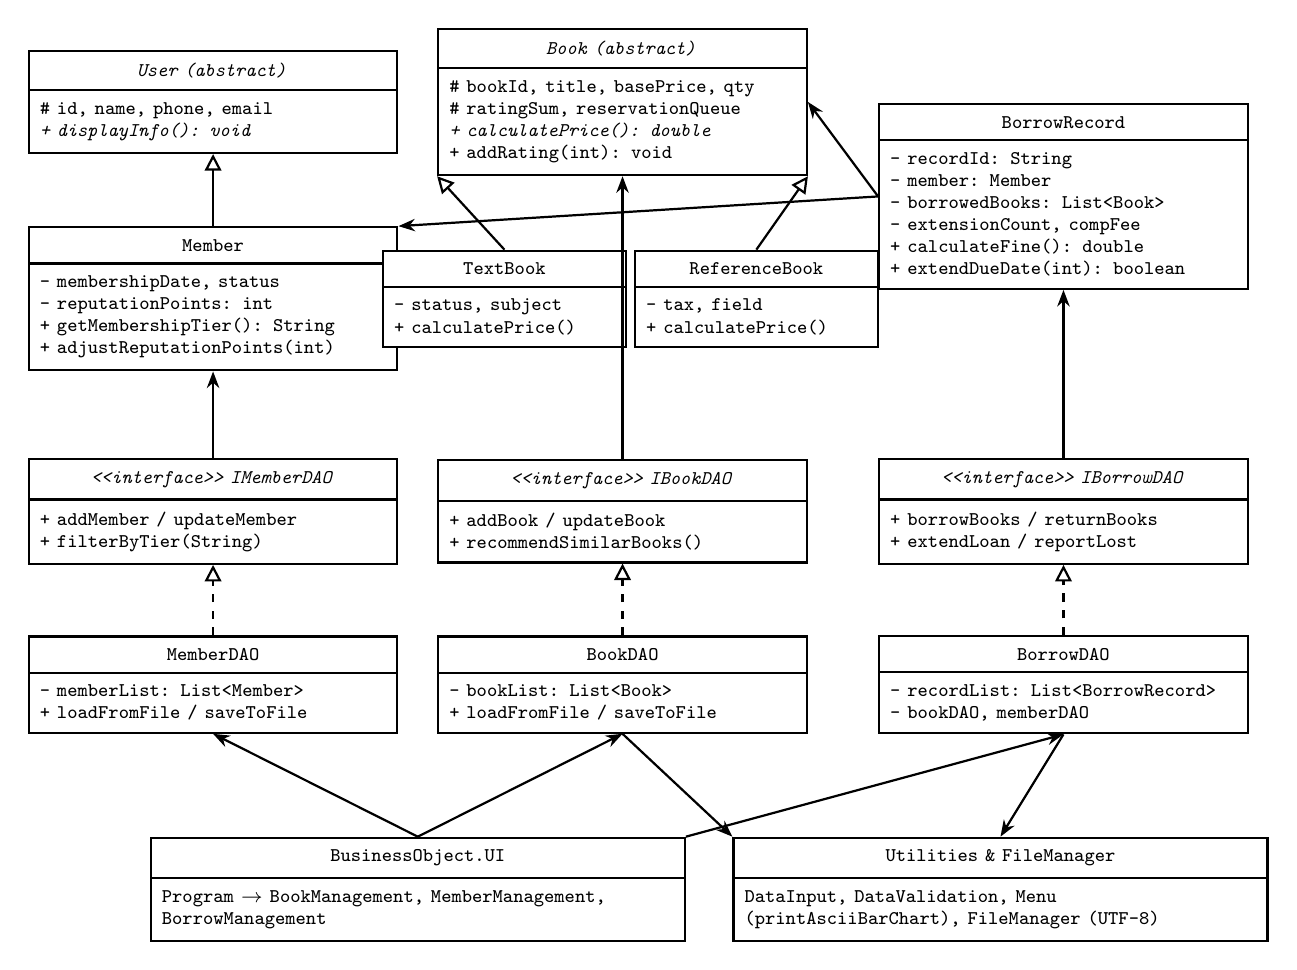
\begin{tikzpicture}[
    pkgbox/.style={
        rectangle split, rectangle split parts=2,
        draw=black, thick, fill=white,
        font=\ttfamily\scriptsize, align=left,
        text width=4.4cm, inner sep=4pt
    },
    inherit/.style={-{Triangle[open, length=6pt, width=6pt]}, thick},
    impl/.style={-{Triangle[open, length=6pt, width=6pt]}, thick, dashed},
    assoc/.style={-{Stealth[length=6pt]}, thick}
]
    % Entities
    \node[pkgbox] (user) at (0, 0) {
        \centerline{\textbf{\textit{User (abstract)}}}
        \nodepart{second}
        \# id, name, phone, email\\
        \textit{+ displayInfo(): void}
    };
    \node[pkgbox] (member) at (0, -2.5) {
        \centerline{\textbf{Member}}
        \nodepart{second}
        - membershipDate, status\\
        - reputationPoints: int\\
        + getMembershipTier(): String\\
        + adjustReputationPoints(int)
    };
    \node[pkgbox] (book) at (5.2, 0) {
        \centerline{\textbf{\textit{Book (abstract)}}}
        \nodepart{second}
        \# bookId, title, basePrice, qty\\
        \# ratingSum, reservationQueue\\
        \textit{+ calculatePrice(): double}\\
        + addRating(int): void
    };
    \node[pkgbox, text width=2.8cm] (tb) at (3.7, -2.5) {
        \centerline{\textbf{TextBook}}
        \nodepart{second}
        - status, subject\\
        + calculatePrice()
    };
    \node[pkgbox, text width=2.8cm] (rb) at (6.9, -2.5) {
        \centerline{\textbf{ReferenceBook}}
        \nodepart{second}
        - tax, field\\
        + calculatePrice()
    };
    \node[pkgbox] (br) at (10.8, -1.2) {
        \centerline{\textbf{BorrowRecord}}
        \nodepart{second}
        - recordId: String\\
        - member: Member\\
        - borrowedBooks: List<Book>\\
        - extensionCount, compFee\\
        + calculateFine(): double\\
        + extendDueDate(int): boolean
    };

    % DAOs
    \node[pkgbox] (imdao) at (0, -5.2) {
        \centerline{\textbf{\textit{<<interface>> IMemberDAO}}}
        \nodepart{second}
        + addMember / updateMember\\
        + filterByTier(String)
    };
    \node[pkgbox] (mdao) at (0, -7.4) {
        \centerline{\textbf{MemberDAO}}
        \nodepart{second}
        - memberList: List<Member>\\
        + loadFromFile / saveToFile
    };

    \node[pkgbox] (ibdao) at (5.2, -5.2) {
        \centerline{\textbf{\textit{<<interface>> IBookDAO}}}
        \nodepart{second}
        + addBook / updateBook\\
        + recommendSimilarBooks()
    };
    \node[pkgbox] (bdao) at (5.2, -7.4) {
        \centerline{\textbf{BookDAO}}
        \nodepart{second}
        - bookList: List<Book>\\
        + loadFromFile / saveToFile
    };

    \node[pkgbox] (ibrdao) at (10.8, -5.2) {
        \centerline{\textbf{\textit{<<interface>> IBorrowDAO}}}
        \nodepart{second}
        + borrowBooks / returnBooks\\
        + extendLoan / reportLost
    };
    \node[pkgbox] (brdao) at (10.8, -7.4) {
        \centerline{\textbf{BorrowDAO}}
        \nodepart{second}
        - recordList: List<BorrowRecord>\\
        - bookDAO, memberDAO
    };

    % UI & Utilities
    \node[pkgbox, text width=6.5cm] (ui) at (2.6, -10.0) {
        \centerline{\textbf{BusinessObject.UI}}
        \nodepart{second}
        \textbf{Program} $\rightarrow$ \textbf{BookManagement}, \textbf{MemberManagement}, \textbf{BorrowManagement}
    };
    \node[pkgbox, text width=6.5cm] (util) at (10.0, -10.0) {
        \centerline{\textbf{Utilities \& FileManager}}
        \nodepart{second}
        \textbf{DataInput}, \textbf{DataValidation}, \textbf{Menu} (\texttt{printAsciiBarChart}), \textbf{FileManager} (UTF-8)
    };

    \draw[inherit] (member) -- (user);
    \draw[inherit] (tb.north) -- (book.south west);
    \draw[inherit] (rb.north) -- (book.south east);
    \draw[assoc] (br.west) -- (member.north east);
    \draw[assoc] (br.west) -- (book.east);

    \draw[impl] (mdao) -- (imdao);
    \draw[impl] (bdao) -- (ibdao);
    \draw[impl] (brdao) -- (ibrdao);

    \draw[assoc] (imdao) -- (member);
    \draw[assoc] (ibdao) -- (book);
    \draw[assoc] (ibrdao) -- (br);

    \draw[assoc] (ui.north) -- (mdao.south);
    \draw[assoc] (ui.north) -- (bdao.south);
    \draw[assoc] (ui.north east) -- (brdao.south);
    \draw[assoc] (bdao.south) -- (util.north west);
    \draw[assoc] (brdao.south) -- (util.north);
\end{tikzpicture}
\end{center}

\textbf{3. OOP Concepts Application Summary}

\begin{itemize}[leftmargin=1.2cm]
    \item \textbf{Encapsulation:} All entity attributes in \texttt{User}, \texttt{Member}, \texttt{Book}, \texttt{TextBook}, \texttt{ReferenceBook}, and \texttt{BorrowRecord} are declared \texttt{private} or \texttt{protected}, and internal \texttt{ArrayList} collections inside \texttt{BookDAO}, \texttt{MemberDAO}, and \texttt{BorrowDAO} are hidden from external classes. State updates occur strictly through validated setters and business methods such as \texttt{adjustReputationPoints()} and \texttt{extendDueDate()}.
    \item \textbf{Inheritance:} \texttt{Member} extends \texttt{User} to inherit personal identity attributes, while \texttt{TextBook} and \texttt{ReferenceBook} extend \texttt{Book} to reuse common bibliographic, rating, and reservation queue fields via \texttt{super(...)}.
    \item \textbf{Polymorphism:} \texttt{TextBook} and \texttt{ReferenceBook} override \texttt{calculatePrice()}, \texttt{displayInfo()}, and \texttt{toFileString()}, enabling \texttt{BookDAO} and \texttt{BorrowRecord} to process mixed book objects polymorphically through \texttt{List<Book>}.
    \item \textbf{Abstraction:} Abstract classes (\texttt{User}, \texttt{Book}) model high-level concepts that cannot be instantiated directly, while DAO interfaces (\texttt{IBookDAO}, \texttt{IMemberDAO}, \texttt{IBorrowDAO}) abstract data storage details away from the UI layer.
\end{itemize}

\textbf{4. CT Skills Evaluation}

\textbf{Decomposition}\\
\textbf{Abstraction}\\
\textbf{Pattern Recognition}\\
\textbf{Generalization}\\
\textbf{Algorithmic Thinking Evaluation \& Iteration}

``I applied \textbf{decomposition} when I separated the system into four distinct packages (\texttt{Core.Entities}, \texttt{DataObjects.DAO}, \texttt{BusinessObject.UI}, and \texttt{Utilities}) and divided the workload evenly across four team members (Member module, Book module, Borrow/Return module, and Infrastructure/Analytics module).\\
I used \textbf{abstraction} by focusing on key attributes required for library operations (such as \texttt{basePrice}, \texttt{quantity}, \texttt{reputationPoints}, \texttt{dueDate}, and \texttt{reservationQueue}) while ignoring irrelevant physical details, and by defining DAO interfaces.\\
I demonstrated \textbf{pattern recognition} in \texttt{BookDAO}, \texttt{MemberDAO}, and \texttt{BorrowDAO} where all three modules share unified CRUD, search, and UTF-8 file persistence methods, as well as in \texttt{Menu.printAsciiBarChart()} which renders proportional bar charts for three different statistical views.\\
I applied \textbf{generalization} by creating the abstract \texttt{Book} and \texttt{User} hierarchies so common attributes and methods are written once and reused across all subclasses.\\
I applied \textbf{algorithmic thinking and iteration} when I reviewed and improved our class diagram and business logic across the four milestones---evolving from basic CRUD operations to multi-criteria \texttt{Comparator} sorting, smart book recommendations, tier-discounted borrowing fees, $150\%$ lost-book compensation, and backward-compatible UTF-8 file parsing.''

\textbf{5. System Testing \& Evidence}

\begin{itemize}[leftmargin=1.2cm]
    \item \textbf{Sample inputs/outputs (Console Dashboard \& ASCII Bar Chart):}
\end{itemize}

\begin{lstlisting}[basicstyle=\ttfamily\scriptsize, backgroundcolor=\color{codebg}, frame=single, rulecolor=\color{codeframe}]
==========================================================================
                BANG TONG HOP TOAN HE THONG (SYSTEM DASHBOARD)
==========================================================================
  [1. KHO SACH]     Tong so dau sach: 10 dau sach (217 cuon ton kho)
                    Tong gia tri tai san kho sach: 36,649,000 VND
  [2. DOC GIA]      Tong so the doc gia: 5 doc gia (VIP: 1 | GOLD: 2 | SILVER: 2)
  [3. MUON - TRA]   Tong so phieu muon: 3 phieu (Dang muon: 2 | Qua han: 2)
                    Phi muon: 130,200 VND | Tien phat: 45,000 VND | Den bu: 0 VND
==========================================================================
  [B001] Lap trinh Huong ... | ##########################            30 cuon
  [B002] Cau truc du lieu... | ######################                25 cuon
  [B003] Co so du lieu qu... | ###################################   40 cuon
  [B006] Clean Code - Ngh... | ##################                    20 cuon
\end{lstlisting}

\begin{itemize}[leftmargin=1.2cm]
    \item \textbf{Explanation of how we tested (3--4 sentences):}
    We tested the system thoroughly by executing both normal end-to-end user workflows and boundary/invalid input test cases across all four subsystems. First, we entered malformed IDs, negative prices, non-numeric strings, and invalid dates to verify that \texttt{DataInput} and \texttt{DataValidation} caught all errors without crashing. Second, we verified polymorphic pricing, VIP/GOLD/SILVER discount rates, due-date extensions (blocking a second extension on the same loan), $150\%$ lost-book penalties, and automatic FIFO reservation alerts when an out-of-stock book is returned. Finally, we restarted the application to confirm that \texttt{Books.txt}, \texttt{Members.txt}, \texttt{BorrowRecords.txt}, and \texttt{Library\_Summary\_Report.txt} preserved all UTF-8 data accurately.
\end{itemize}

\textbf{6. Self-Evaluation (Strengths \& Limitations)}

``One strength of my system is its clean 4-layer OOP architecture combined with seven practical creative features: automated Membership Tiers (\texttt{VIP}/\texttt{GOLD}/\texttt{SILVER}) \& Reputation Points, Star Ratings ($1\text{--}5\star$) \& Smart Book Recommendations, FIFO Reservation Queues, Loan Extensions ($+7$ days), $150\%$ Lost/Damaged Book Compensation, Console ASCII Bar Charts, and automated Receipt/Report file exporting.\\
However, a limitation is that the application currently operates as a single-user console program storing data in flat text files (\texttt{.txt}) without multi-user concurrency or database transactions.\\
In the future, I can improve by migrating the DAO layer to a relational database (SQL Server/MySQL via JDBC), refactoring traditional loops and anonymous \texttt{Comparator} classes to Java 8+ Lambda Expressions and Stream API, and developing a JavaFX graphical user interface.''

\textbf{7. Final Reflection (6--8 sentences)}

``Completing the Library Management System across all four milestones significantly strengthened my practical command of Object-Oriented Programming and Computational Thinking. From OOP, I learned how Encapsulation protects domain invariants, how Inheritance eliminates duplicate code, and how Polymorphism and Abstraction decouple high-level business workflows from concrete subclass details. My Computational Thinking skills improved markedly as our team practiced Decomposition to split the project into four independent modules and Pattern Recognition to standardize DAO interfaces and input validators. Designing algorithms for smart book recommendations, overdue fine calculation, reputation tier discounts, and ASCII bar chart scaling also sharpened my algorithmic thinking. Furthermore, integrating UTF-8 File I/O with defensive \texttt{try-catch} blocks taught me how to build resilient software that recovers gracefully from bad inputs or missing files. Next time, I would establish the final file serialization schema and cross-module interface signatures even earlier in Week 1 so that team integration goes even faster.''

\end{document}
